\documentclass{article}
\usepackage[utf8]{inputenc}
\usepackage{amsmath}
\usepackage{graphicx}
\usepackage{geometry}
\usepackage[english, french]{babel}
\graphicspath{{images/} 
\geometry{legalpaper, lmargin=0.7in, bmargin=1in}}
\selectlanguage{french}

\setlength\parindent{0pt}% globally suppress indentation

\begin{document}
%%%%%%%%%%%%%%
%page  titre en caractères plus large
%%%%%%%%%%%%%%
\begin{titlepage}   
	\large{
		\begin{center}
			UNIVERSITÉ DE SHERBROOKE\\Faculté de génie\\
			Département de génie électrique et génie informatique\\
			\vspace{3cm}
			{\LARGE\textbf{Principes de dynamique et méthodes numériques}}\\
			\vspace{2cm}
			\LARGE{Rapport APP2}\\
			\vspace{2cm}
			Présenté à\\l'équipe professorale de la session S4\\
			\vspace{2cm}
			Produit par\\Éric Beaudoin, Alexandre Gagnon, Philippe Garneau\\
			\vspace{1cm}
			\vfill{23 mai 2017 - Sherbrooke}
		\end{center}
	}
\end{titlepage}
\newpage
%%%%%%%%%%%%%%
%Table des matières
%%%%%%%%%%%%%%
\tableofcontents

\newpage
\section{Introduction}
THIS NEEDS TO BE CHANGEDDDD
Dans le cadre de l'implémentation d'un système de commande du bras mécanique de l'entreprise CRM, il faut analyser le mouvement d'un point A sur le plan 2D de celui-ci. Le point A, situé à l'extrémité des bras du robot, bouge selon le bras BA attaché au moteur MB et le bras BA bouge selon le bras OB avec le moteur MO. Notre mandat est de déterminer les forces et les couples nécessaires pour maintenir le robot en équilibre ou de le bouger selon des directives spécifiques. Pour la résolution de la problématique, l'équipe a divisée l'ensemble en plusieurs étapes. La première étape fût de regarder la cinématique du système de manière générale, ensuite dans des cas avec des restrictions sur les mouvements possibles du point A dans le plan 2D. En deuxième partie, l'analyse est centrée sur la statique et la dynamique du système. 

\section{Design de la trajectoire et du débit d'eau}
\subsection{Hauteur de $y_f$ et coefficients du polynôme d'interpolation de la trajectoire}
Afin de trouver la valeur de $y_f$, plusieurs étapes ont été nécessaires. En premier lieu, nous avons trouvé tous les polynômes d'interpolation de la trajectoire avec des valeurs de $y_f$ allant de 10m à 15m en incréments de 0.1m. Ensuite, nous avons fait la dérivée de  chaque polynôme et avons vérifié la valeur de celle-ci à la fin de la glissade, donc à x=25m. Nous avons sauvegardé toutes les valeurs de $y_f$ ayant un résultat de dérivée à $x=25m$ entre -0.01 et 0.01 et après avoir fait la moyenne de ces résultats, nous avons trouvé une valeur de $y_f=12.27m$. Le polynôme d'interpolation final de la trajectoire est:
\begin{equation}
y = 30-4.6001x+0.6310x^2-0.0329x^3+0.0006x^4
\end{equation}

\subsection{Vitesse de sortie du participant au point E sans friction}
Afin de trouver la vitesse de sortie du participant au point E, il faut utiliser la loi de conservation de l'energie mecanique. Nous savons qu'il n'y a pas de force non-conservatives qui agissent sur notre systeme dans ce cas, donc l'equation est:
\begin{equation}
	\Delta E_p + \Delta E_c = 0
\end{equation}

\begin{equation}
	mg\Delta h + \frac{1}{2}m\Delta v^2 = 0
\end{equation}

\begin{equation}
	784.8(12.27-30) + 40(v-0)^2 = 0
\end{equation}

\begin{equation}
	v = 18.65 m/s = 67.14 km/h
\end{equation}
En observant ce résultat, il est évident qu'une force de friction sera nécessaire afin de ralentir le participant pour ne pas dépasser les contraintes définies dans le devis.

\subsection{Ordre et coefficients du polynôme d'approximation de $\mu_f$}
Afin de trouver une bonne approximation de la relation entre le coefficient de friction et le pourcentage d'ouverture de la valve, nous avons utilisé la projection orthogonale. Pour chaque valeur de $M$ allant de $N-3$ à 1 où $N=11$, nous avons généré une matrice de bonne grandeure pour ensuite trouver le polynôme d'approximation complet et finalement trouvé la valeur du $RMS$. Après avoir tracé les 8 courbes et analysé les valeurs de $RMS$, il peut être observé que les polynômes pour $M=4,5,6,7$ ont un $RMS$ très similaire. Par contre, les courbes pour $M=4,6,7$ démontrent un comportement où le coefficient de friction augmente lorsque le pourcentage d'ouverture de la valve augmente, donc ces polynômes sont ignorés. La courbe restante est celle où $M=5$ et nous donne un polynôme d'ordre 4 qui est:
\begin{equation}
	\mu_f = 0.8691608391-0.0090679875x+0.0000287878x^2+0.0000005633x^3-0.0000000035x^4 
\end{equation}
La valeur du $RMS$ pour ce polynôme est $0.0176219$.

\subsection{Coefficient de friction dynamique}
hello hello je trouve le coefficient

\subsection{Ouverture de la valve en \% pour $\mu_f=0.63$}
Connaissant le coefficient de friction désiré, il faut simplement utiliser la fonction $roots()$ avec le polynôme d'approximation de $M=5$ pour trouver la valeur de l'ouverture de la valve en \%. La fonction $roots()$ nous donne quatre (4) résultats, mais on observe qu'un seul résultat nous donne une valeur infiérieure à 100, donc on ignore les autres. Le pourcentage d'ouverture de la valve pour $\mu_f=0.63$ est:
\begin{equation}
	ouverture = 30.88\%
\end{equation}

\subsection{Vitesse du participant le long de la trajectoire}
Pour trouver le graphique de la vitesse du participant le long de la trajectoire, il faut utiliser la loi de conservation de l'énergie mécanique. Nous pouvons prendre l'équation suivante:
\begin{equation}
	\Delta E_p + \Delta E_c = -\mu_fmgx
\end{equation}
Pour résoudre cette équation, il faut trouver une relation entre la hauteur du participant et sa position en x. Cette relation est exprimée par le polynôme d'interpolation trouvé précédemment. L'équation pour trouver la vitesse par rapport à la position du participant est:
\begin{equation}
	v = \sqrt{2(-xg\mu_f-g(-4.6001x+0.6310x^2-0.0329x^3+0.0006x^4))}
\end{equation}
Cette équation donne le graphique suivant:
\begin{center}
  \makebox[\textwidth]{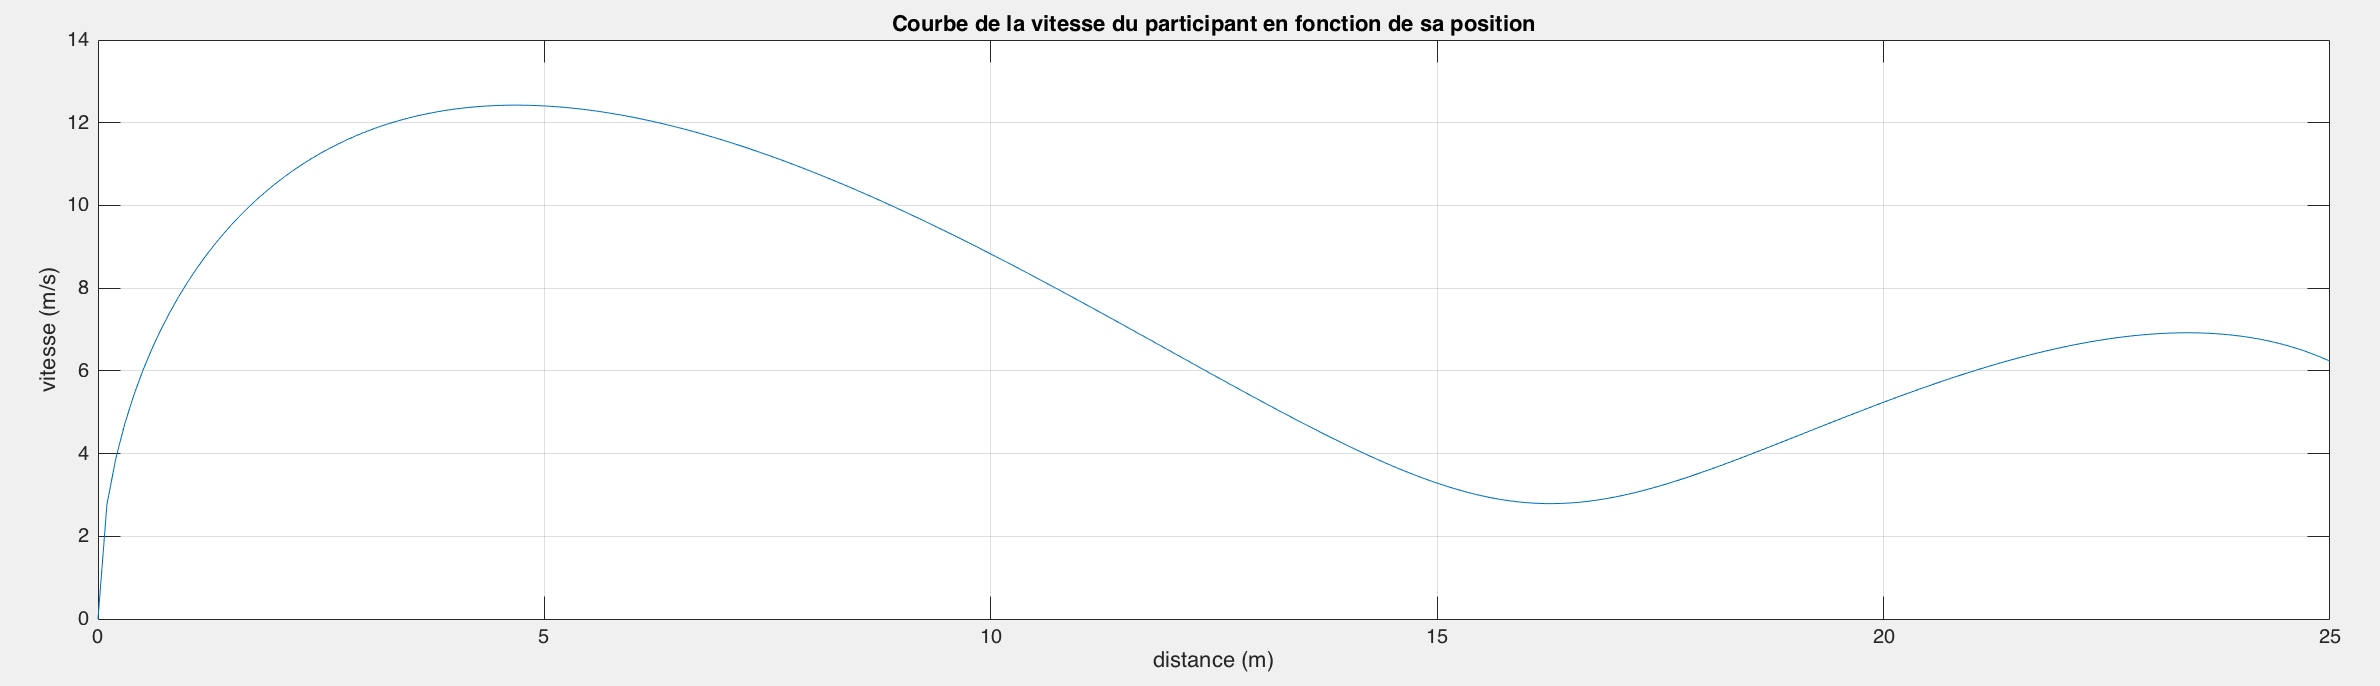
\includegraphics[width=\linewidth]{vit_pos}}
\end{center}

 
 \subsection{minuterie}
 Pour la situation G1, le coefficient de restitution = 0 et
 en utilisant les formules de conservation de l'energie 
 
 \begin{equation}
 m_{a}V_{a}^{n} + m_{b}V_{b}^{n} =( m_{a} + m_{b})V_{ab}^{'n} 
 \end{equation}
 \begin{equation}
 e = \frac {V_{B}^{'n}-V_{A}^{'n}}{V_{A}^{n}-V_{B}^{n}} 
\end{equation}  

 On détermine, sachant que $ e = 0$, $ V_{A}^{n}$ = 22,5 km/h et que  $V_{B}^{n}$ = 3,6 km/h on trouve rapidement
 \begin{equation}
  80*22,5 +8*-3,6 = 88(V_{ab}^{'n})
\end{equation}  
donnant

\begin{equation}
V_{ab}^{'n} = 20,127 km/h * (3600sec/1000m) = 5.59 m/s
\end{equation}


\vspace*{4mm}
 Pour la situation G2, ou le coefficient de restitution = 0.8 On développe comme suit:

 \begin{equation}
 0,8 = \frac{V_{B}^{'n}-V_{A}^{'n}}{26,1}
\end{equation} 
 \begin{equation}
 20.88 = V_{B}^{'n}-V_{A}^{'n} 
\end{equation} 
En réarrangant l'équation (10) , on obtient:
 \begin{equation}
 221,4 = 10V_{ab}^{'n}+V_{B}^{'n}
\end{equation} 

on isole  $V_{B}^{'n} = 221,4 - 10V_{A}^{'n}$ de l'équation (16) et en la remplaçant dans l'équation (15), on arrive au résultat suivant :
\begin{equation}
  20,88 = {221,4 - 10V_{A}^{'n}-V_{A}^{'n}}
\end{equation}

\begin{equation}
  V_{A}^{'n} = 18,229 Km/h *(3600sec/1000m) = 5,06 m/s
\end{equation}
\vspace*{4mm}

Sachant tout cela, nous pouvons trouver le temps que prennent le participant pour franchir la distance de 3m dans les deux cas. Pour le cas G1, avec incertitude de 0,02sec, on obtiens un résultat de 0,54 sec pour quitter la surface de la plaque de 3m et pour G2, 0,59 sec. On peut donc choisir la moyenne comme temp de minuterie nous donnant un $\Delta t_{m}$ 0,565 sec.
 
 
 \subsection{coussin trampoline}
 
 EN se basant sur la formule de l<acceleration gravitationelle et de la formule des ressorts, on trouve facilement le $\Delta x$ en resolvant lequation quadratique que donne notre developpement
 
 \begin{equation}
\ mg \Delta h = \frac{1}{2}k \Delta x ^2
 \end{equation}
 \begin{equation}
 88*9,81*(5+\Delta x) = \frac{1}{2}*6000*\Delta x^2 
 \end{equation}
 \begin{equation}
 0 = 3000\Delta x^2 - 863.28 \Delta x - 4316.4 \quad nous\quad  donnant\quad  un\quad  \Delta x=\quad 1.35m 
 \end{equation}

\subsection{bassin}

on début avec l'équation donner dans l'énoncé
\begin{equation}
\ m \frac{dv}{dt} = \sum F = mg - K_{f}mg - bv^2
\end{equation}
comme dictée par la 2e loi de Newton:
\begin{equation}
\ \frac{dv}{dt} = \frac{dv}{dz} \frac{dz}{dt} = v\frac{dv}{dz}
\end{equation}
en faisant la substitution pr/c/dente, en regroupant les terme et en divisant les deux cote par v on obtiens:
\begin{equation}
\ m\frac{dv}{dz} =  \frac{mg ( 1- K_{f})}{v} - bv
\end{equation}
On pose donc l'accélération a zero pour avoir le systèeme a l'équilibre nous donnant l'équation 57
\begin{equation}
\ 0 =  mg ( 1- K_{f}) - bv_{e})
\end{equation}

\begin{equation}
\ v_{e} = \sqrt{\frac{mg(1-K_{f})}{b}}
\end{equation}

par la suite on doit linéariser notre équation 55 pour pouvoir facilement isoler notre z. On commence par linéarisser notre seul terme non lineaire etant 

\begin{equation}
\ \frac{mg ( 1- K_{f})}{v} = \frac{mg}{v_{e}}(1-K_{f})+
\Bigg[\begin{array}{cc}
    \frac{-1}{V_{e}^2}mg(1-K_{f})
    \end{array}\Bigg]
    (v-v_{e})
\end{equation}
en remplacant le tout dans lequation de base 55
\begin{equation}
mv \frac{dv}{dz} = mg - \Bigg[\begin{array}{cc}
\frac{mg}{v_{e}}(1-K_{f})+
\Bigg[\begin{array}{cc}
    \frac{-1}{V_{e}^2}mg(1-K_{f})
    \end{array}\Bigg]
    (v-v_{e}) \end{array}\Bigg] - bv
\end{equation}
comme la on sait que
\begin{equation}
\Delta v = v - v_{e}  \quad  \textrm{donc} \quad    v = \Delta v+ v_{e}
\end{equation}

et que lon sosutrait les terme de l'equation a lequilibre on obtiens l'equation lineaire  ( en isolant les v et le z de chaque coté ):

\begin{equation}
\ m \frac{d \Delta v}{\Delta v}= \Bigg[\begin{array}{cc} \frac{1}{m} \Bigg[\begin{array}{cc}
    \frac{-1}{V_{e}^2}mg(1-K_{f})
    \end{array}\Bigg]  - b\end{array}\Bigg] d_{z}
\end{equation}

par la suite, on intègre chaque côté de l'équation. Comme le coté gauche est bornée de 0,1ve jusqu'a vi - ve, cela nous donne 4,9644. Comme le côté droit ne contient qu'une variable étant le dz qui deviendras $\Delta$ z
 Le reste du calcul effectuer sur matlab nous donne un z de 4,23m car 
 \begin{equation}
 4,9644 = \Bigg[\begin{array}{cc} \frac{1}{80} \Bigg[\begin{array}{cc}
    \frac{-1}{0,913^2}80*9.81(1-0,95)
    \end{array}\Bigg]  - 47\end{array}\Bigg] \Delta z
 \end{equation}
 
 


\end{document}
